\documentclass[11pt,a4paper]{article}
\pdfinfoomitdate=1
\pdftrailerid{}
\pdfsuppressptexinfo=15
\usepackage[margin=24mm]{geometry}
\usepackage[T1]{fontenc}
\usepackage[utf8]{inputenc}
\usepackage{lmodern,amsmath,amssymb,booktabs,longtable,array,graphicx,microtype}
\usepackage{xurl}
\usepackage[hidelinks]{hyperref}
\usepackage{placeins}
\setlength{\emergencystretch}{3em}
\setlength{\parskip}{4pt}
\setlength{\parindent}{0pt}
\allowdisplaybreaks
\title{AE4 control of salivary transport:\\full system mathematics and parameter dependence}
\author{Tasks 44 and 45: standalone technical analysis}
\date{15 September 2026}
\begin{document}
\maketitle
\begin{abstract}
The frozen Task 40 system is analysed without removing intracellular or
luminal carbon, alkalinity, volume, pH closure, electrical closure or AE4
regulation. Exact charge elimination leaves eleven independent dynamic
coordinates. We prove conditional closure and balance results and distinguish
them from local equilibrium calculations and finite time simulations. Equal
cation routing cancels the explicit AE4 cycle in one stationary chloride
balance; it does not cancel state mediated secretion sensitivity. The parent
system has slow local modes of approximately 346 s in WT and 460 s in the
AE4 null. A physiological NBC absent root exists at reduced AE4 loading,
qualifying any universal necessity claim. Within the prescribed target selected
Task 41 family, the first numerical crossing of a 30.3\% cumulative deficit
requires approximately 89.51\% AE4 dependent stimulated CaCC recruitment.
That family passes the inherited 600 s gates but later violates the pH gate.
Local sensitivity identifies pump, NBC and NKCC capacities, CaCC recruitment
and finite buffering as priorities for independent constraint. Unknown parameter
ranges, thermodynamic tensions and experimental discrepancies prevent global
robustness or mechanism validation claims.
\end{abstract}

\section{Scope, checkpoint continuity and interpretation}
This report continues the existing branch
\texttt{analysis/task-44-full-system-mathematics}, recovered at
\nolinkurl{b7b775a0277d93263c4de339745806e5658ec9c2}.
The complete numerical checkpoint independently replayed for this report is
\nolinkurl{f783785a863440df459e9c5530beba4c7eb59110}.
Task 43 remains on the separate, unmerged parameter provenance branch; its
final report checkpoint is
\nolinkurl{bc3e37645b9a7519dee0da9d1e2df55e291dd983}.
The companion crosswalk reads numerical results at the exact Task 44 commit,
with source file hashes. Neither a fit nor a new production model is introduced.

The archived \texttt{Marty.tex} fixes intracellular concentrations other than
sodium, potassium and chloride, lumen concentrations, membrane potentials
and cell volume. Those assumptions remove precisely the carbon, alkalinity,
storage and osmotic responses at issue here. Its reduction is therefore not
reused. The following scaling is an invertible coordinate change; every
retained degree of freedom remains dynamic or is reconstructed by an exact
constraint. The inherited algebraic electrical approximation is identified
as an assumption, not justified retrospectively by a nonexistent capacitance
parameter.

The report uses four levels of conclusion. A proved identity is conditional
on its stated equations and domain. A local numerical result applies at the
specified parameter point and branch of roots. A finite time numerical result
applies to its stated stimulus, initial state and observation window.
Unresolved questions include biological mechanism identity, global uniqueness,
global stability, uncertainty ranges and robustness over those ranges.

% Self-contained mathematical sections, included by report.tex.
\section{The retained system and exact scaling}
\label{sec:exact-full-system}
The analysis keeps the intracellular and luminal amounts of sodium,
potassium, chloride, total inorganic carbon and total alkalinity; both
volumes; and the AE4 regulatory fraction.  Carbonate speciation and two
membrane voltages are recovered algebraically at every evaluation.
The older reduction in \texttt{Marty.tex} is therefore not used: neither a
fixed pH nor a fixed volume can be inserted into the following identities.
Alkalinity is a conserved acid--base coordinate, not bicarbonate alone.

Let $N,H,E,B,J_4$ denote inward NKCC1 cycles, NHE1 sodium uptake with proton
extrusion, AE2 chloride uptake with bicarbonate extrusion, NBC cycles and
AE4 cycles respectively.  A positive NBC cycle imports one sodium and two
bicarbonates.  Write $P=P_a+P_b$ for the total pump cycles,
$K_a,K_b$ for potassium efflux from cell to lumen and bath, and $C_a$ for
chloride efflux from cell to lumen.  The paracellular flux $j_{p,s}$ is
positive from lumen to bath for species $s$.  The carbon dioxide fluxes
$D_b,D_a$ are positive from bath and lumen into the cell.  Water fluxes
$q_b,q_a,q_t,Q$ are positive from bath to cell, cell to lumen, bath to lumen,
and lumen to sink respectively.  These are signed fluxes, not their positive
parts.  The general AE4 source vector is
\[
 \nu=(\nu_{\mathrm{Na}},\nu_{\mathrm K},\nu_{\mathrm{Cl}},\nu_T,\nu_A),
 \qquad S^4=J_4\nu .
\]

Take $C_0=[\mathrm{Na}]_e$, $V_0=V_i(0)$, $L_0=V_l(0)$ and the initial
stimulated WT NKCC1 \emph{cycle} flux $J_0$.  Define
\[
 t_0=\frac{C_0V_0}{J_0},\quad \tau=t/t_0,\quad
 \varepsilon=L_0/V_0,\quad v=V_i/V_0,\quad \ell=V_l/L_0,
 \quad x_s=\frac{n_{s,i}}{C_0V_0},\quad y_s=\frac{n_{s,l}}{C_0L_0}.
\]
Every ionic or carbon flux below is divided by $J_0$, and every water flux
by $J_0/C_0$; a hat marks these fluxes.  Dimensionless concentrations are
$c_{s,i}=x_s/v$ and $c_{s,l}=y_s/\ell$.  Primes mean $d/d\tau$.
The full dimensionless amount and volume equations are
\begin{align}
 x_{\mathrm{Na}}'&=\widehat N+\widehat H+\widehat B+
                \nu_{\mathrm{Na}}\widehat J_4-3\widehat P,\notag\\
 x_{\mathrm K}'&=\widehat N+\nu_{\mathrm K}\widehat J_4+
                2\widehat P-\widehat K_a-\widehat K_b,\notag\\
 x_{\mathrm{Cl}}'&=2\widehat N+\widehat E+
                \nu_{\mathrm{Cl}}\widehat J_4-\widehat C_a,\notag\\
 x_T'&=-\widehat E+2\widehat B+\nu_T\widehat J_4+
                \widehat D_b+\widehat D_a,\notag\\
 x_A'&=\widehat H-\widehat E+2\widehat B+\nu_A\widehat J_4,\notag\\
 v'&=\widehat q_b-\widehat q_a,\label{eq:dimless-cell}\\
 \varepsilon y_{\mathrm{Na}}'&=3\widehat P_a-\widehat j_{p,\mathrm{Na}}
                -\widehat Q c_{\mathrm{Na},l},\notag\\
 \varepsilon y_{\mathrm K}'&=-2\widehat P_a+\widehat K_a-
                \widehat j_{p,\mathrm K}-\widehat Qc_{\mathrm K,l},\notag\\
 \varepsilon y_{\mathrm{Cl}}'&=\widehat C_a-\widehat j_{p,\mathrm{Cl}}
                -\widehat Qc_{\mathrm{Cl},l},\notag\\
 \varepsilon y_T'&=-\widehat j_{p,\mathrm{HCO}_3}-\widehat D_a-
                \widehat Qc_{T,l},\notag\\
 \varepsilon y_A'&=-\widehat j_{p,\mathrm{HCO}_3}-\widehat Qc_{A,l},\notag\\
 \varepsilon\ell'&=\widehat q_a+\widehat q_t-\widehat Q,
 \qquad \theta_4 r'=\beta-r,\qquad \theta_4=30/t_0.
 \label{eq:dimless-lumen}
\end{align}
The neutral manifold is
\begin{equation}
 x_A=x_{\mathrm{Na}}+x_{\mathrm K}-x_{\mathrm{Cl}}-a_f,
 \quad y_A=y_{\mathrm{Na}}+y_{\mathrm K}-y_{\mathrm{Cl}},
 \quad a_f=\frac{n_{\mathrm{fixed}}}{C_0V_0}.
 \label{eq:neutral-manifold}
\end{equation}
Eliminating these two amounts leaves eleven independent dynamic
coordinates.  This is exact: cell charge is conserved; luminal charge obeys
$\dot q_l=-Qq_l/V_l$ and hence remains zero from zero initial charge.
Alkalinity and its effect on pH remain in the reconstructed state.

\subsection{Dimensionless constitutive laws}
Here $h_i$ and $b_i$ denote the dimensionless hydrogen and bicarbonate
concentrations from the carbonate closure below.  All half concentrations
and dissociation constants in this subsection are divided by $C_0$;
numerical rate constants retain their declared unit conversions.
For constant full stimulation the frozen NKCC1 and NHE1 multipliers are
$m_N=1.75$ and $m_H=2.3$.  More generally their separate clipped calcium
coordinates have the frozen endpoints used by the production objects:
the active NKCC1 endpoints are $0.058$ and $0.1\,\mu\mathrm M$,
whereas NBC and NHE1 use $0.058$ and $0.25\,\mu\mathrm M$.
This distinction matters away from full stimulation.

Put $X=c_{\mathrm{Na},i}c_{\mathrm K,i}c_{\mathrm{Cl},i}^{2}$.  The
Palk law actually selected in Task 40~\cite{Palk2010} is
\begin{equation}
 \widehat N=e_Nm_N\frac{\alpha_N A_1}{J_0A_3}
   \frac{1-\eta_2X}{1+\eta_4X},\qquad
 \eta_2=\frac{A_2C_0^4}{A_1},\quad
 \eta_4=\frac{A_4C_0^4}{A_3}.
 \label{eq:dimless-nkcc}
\end{equation}
The coefficients are $A_1=157.5$, $A_2=2.0096\,10^{-5}$,
$A_3=1.0306$ and $A_4=1.3852\,10^{-6}$ in the repository's mM
convention.  The effective amount flux $\alpha_N$ comes from the frozen
WT calibration, not an imported membrane density.

For NHE1, choose $k_*=1000k_{1+}$, converting its printed rate per
millisecond into a rate per second.  Let barred rates be divided by $k_*$:
\begin{align*}
 \bar a&=\frac{1000k_{1+}}{k_*}
       \frac{c_{\mathrm{Na},e}}{c_{\mathrm{Na},e}+K_{\mathrm{Na},e}}
       \frac{K_{H,e}}{h_e+K_{H,e}},&
 \bar b&=\frac{1000k_{2+}}{k_*}
       \frac{h_i}{h_i+K_{H,i}}
       \frac{K_{\mathrm{Na},i}}{c_{\mathrm{Na},i}+K_{\mathrm{Na},i}},\\
 \bar c&=\frac{1000k_{1-}}{k_*}
       \frac{c_{\mathrm{Na},i}}{c_{\mathrm{Na},i}+K_{\mathrm{Na},i}}
       \frac{K_{H,i}}{h_i+K_{H,i}},&
 \bar d&=\frac{1000k_{2-}}{k_*}
       \frac{h_e}{h_e+K_{H,e}}
       \frac{K_{\mathrm{Na},e}}{c_{\mathrm{Na},e}+K_{\mathrm{Na},e}}.
\end{align*}
Thus, with the exact printed Cha constants selected by production~\cite{Cha2009},
\[
 M_H=\frac{1}{1+(1+h_e/K_{M,e})(K_{M,i}/h_i)^3},\quad
 \widehat H=\frac{n_Hk_*}{J_0}e_Hm_HM_H
        \frac{\bar a\bar b-\bar c\bar d}{\bar a+\bar b+\bar c+\bar d}.
\]
The printed $k_{2-}=183\,\mathrm{ms}^{-1}$ is retained: the small
rounding discrepancy in microscopic reversibility is not silently repaired.
The other acid--base flux laws are
\begin{align*}
 \widehat E&=e_2\gamma_2\tanh\left[
  \frac{\log(c_{\mathrm{Cl},e}b_i/(c_{\mathrm{Cl},i}b_e))}{w_2}\right],
 &\gamma_2&=G_2/J_0,\\
 \widehat B&=\gamma_Bu\tanh\left[
  \frac{\log(c_{\mathrm{Na},e}b_e^2/(c_{\mathrm{Na},i}b_i^2))+\psi_b}{w_B}\right],
 &\gamma_B&=G_B/J_0,\\
 \widehat D_b&=\delta_b(c_{\mathrm{CO}_2,e}-c_{\mathrm{CO}_2,i}),
 &\widehat D_a&=\delta_a(c_{\mathrm{CO}_2,l}-c_{\mathrm{CO}_2,i}).
\end{align*}
Here $\delta_{a,b}=P_{\mathrm{CO}_2,a,b}C_0/J_0$,
$\psi_b=V_b/V_T$, $V_T=RT/F$, and $u$ is the frozen NBC calcium
coordinate.  The tanh widths are dimensionless effective parameters.

For the inherited AE4 shared carrier, write $k_4$ for its common chloride
attempt rate.  Define
\begin{align*}
 L_c&=\log(c_{\mathrm{Cl},e}/c_{\mathrm{Cl},i}),&
 L_s&=\log(c_{s,i}/c_{s,e})+2\log(b_i/b_e),\quad s\in\{\mathrm{Na},\mathrm K\},\\
 a_c^\pm&=\exp(\pm L_c/2),&
 a_s^\pm&=(k_s/k_4)\exp(\pm L_s/2),\\
 U&=a_c^++a_{\mathrm{Na}}^-+a_{\mathrm K}^-,&
 W&=a_c^-+a_{\mathrm{Na}}^++a_{\mathrm K}^+,\quad
 \pi_i=U/(U+W),\quad\pi_o=W/(U+W).
\end{align*}
The scalar cycle is exactly
\[
 \widehat J_4=e_4\gamma_4(1+0.25r)
 \left[(a_{\mathrm{Na}}^++a_{\mathrm K}^+)\pi_i
       -(a_{\mathrm{Na}}^-+a_{\mathrm K}^-)\pi_o\right],
 \qquad\gamma_4=n_4k_4/J_0.
\]
The frozen cooperative gate is absent.  Task 40 applies equal ensemble
sodium and potassium routing to this scalar cycle.  The seven Catal\'an
classes change its source vector but do not provide new class specific
kinetics.  Local detailed balance of the inherited carrier edges does not
by itself establish thermodynamic consistency of those substituted vectors.

To specify the electrical laws, scale each conductance $G$ as
$g=GV_T10^{15}/(FJ_0)$.  The reversal potential for a valence $z_s$ is
$e_{s,uv}=z_s^{-1}\log(c_{s,v}/c_{s,u})$.  With
$g_{K,a},g_{K,b},g_{C,a}$ incorporating the frozen calcium gate
$a_{\mathrm{Ca}}$ and background conductances, explicitly
\[
 g_{K,a}=g_{K,\mathrm{total}}a_{\mathrm{Ca}}f_K+g_{a,\mathrm{bg}},\quad
 g_{K,b}=g_{K,\mathrm{total}}a_{\mathrm{Ca}}(1-f_K)+g_{b,\mathrm{bg}},\quad
 g_{C,a}=g_{\mathrm{Cl},a}a_{\mathrm{Ca}},
\]
the channel and paracellular fluxes are
\begin{align*}
 \widehat K_a&=g_{K,a}(\psi_a-e_{K,il}), &
 \widehat K_b&=g_{K,b}(\psi_b-e_{K,ie}),\\
 \widehat C_a&=-g_{C,a}(\psi_a-e_{\mathrm{Cl},il}), &
 \widehat j_{p,s}&=\frac{g_{p,s}}{z_s}
   (\psi_b-\psi_a-e_{s,le}).
\end{align*}
The apical pump is
\[
 \widehat P_a=\gamma_P f_P
 \frac{c_{\mathrm{Na},i}^3}{c_{\mathrm{Na},i}^3+K_{P,\mathrm{Na}}^3}
 \frac{c_{\mathrm K,l}^2}{c_{\mathrm K,l}^2+K_{P,\mathrm K}^2},
 \qquad\gamma_P=G_P/J_0,
\]
and the basolateral expression replaces $f_P,c_{\mathrm K,l}$ by
$1-f_P,c_{\mathrm K,e}$.  These pump rates are voltage independent in the
frozen model.  The calcium gate is $c_{\mathrm{Ca}}^n/(c_{\mathrm{Ca}}^n+K_{\mathrm{Ca}}^n)$,
using the same calcium units in numerator and denominator.

For water define dimensionless osmolarities
\[
 o_i=c_{\mathrm{Na},i}+c_{\mathrm K,i}+c_{\mathrm{Cl},i}+c_{T,i}
       +(\beta_i+\iota_i)/v,\quad
 o_l=c_{\mathrm{Na},l}+c_{\mathrm K,l}+c_{\mathrm{Cl},l}+c_{T,l},
\]
where $\beta_i=n_{\mathrm{buffer},i}/(C_0V_0)$ and
$\iota_i=n_{\mathrm{other\ impermeant}}/(C_0V_0)$.  The bath expression
includes its declared untracked osmolyte concentration.  Exactly as in the
production law, free hydrogen and hydroxide are omitted from osmolarity,
and the tiny luminal buffer is not added as an osmotic particle.  No new
approximation is introduced by the present scaling.  Then
\[
 \widehat q_b=\lambda_b(o_i-o_e),\quad
 \widehat q_a=\lambda_a(o_l-o_i),\quad
 \widehat q_t=\lambda_t(o_l-o_e),\quad
 \widehat Q=\omega\varepsilon(\ell-d_l)_+,
\]
with $\lambda_j=L_jC_0^2/J_0$, $\omega=k_{\mathrm{out}}t_0$,
and $d_l=V_{\mathrm{dead}}/L_0$.  These equations close
\eqref{eq:dimless-cell}--\eqref{eq:dimless-lumen} without fixing a volume,
composition, carbon pool or voltage.

\section{Carbonate closure and pH derivatives}
\label{sec:carbonate-proof}
Write $p$ for pH, $h=10^{-p}$ in molar units,
$K_1=10^{-pK_1}$ and $K_2=10^{-pK_2}$.  The carbonate fractions are
\[
 (\alpha_0,\alpha_1,\alpha_2)=
 \frac{(h^2,K_1h,K_1K_2)}{h^2+K_1h+K_1K_2},\qquad
 f(p)=\alpha_1+2\alpha_2,\quad
 g(p)=\frac1{1+10^{pK_b-p}}.
\]
In concentration units mM let
$w(p)=10^3(10^{p-pK_w}-10^{-p})=[\mathrm{OH}]-[\mathrm H]$.
For either compartment, with fixed finite buffer amount $n_b$, the closure
is the single equation
\begin{equation}
 G(p;n_T,n_A,V)=n_Tf(p)+n_bg(p)+Vw(p)-n_A=0.
 \label{eq:carbonate-amount}
\end{equation}
Equivalently, for the cell,
$x_A=x_Tf(p)+\beta_i g(p)+v w(p)/C_0$; the lumen uses $y_T,y_A,\ell$
and $\beta_l=n_{b,l}/(C_0L_0)$.  Thus dilution of the finite buffer is
retained exactly.

\paragraph{Proposition: unique speciation on the stated domain.}
Suppose $V>0$, $n_T\geq0$, $n_b\geq0$, and all constants are finite and
strictly positive in their concentration representation.  For each real
$n_A$, equation \eqref{eq:carbonate-amount} has exactly one real pH.
The solution depends smoothly on the retained amounts and volume on their
open physical domain.  For the production implementation one additionally
requires $n_T>0$ and
\[
 G(p_{\min})\leq0\leq G(p_{\max});
\]
smoothness within the executable domain is asserted with strict bracket
inequalities.  This numerical bracket is distinct from a physiological
pH acceptance interval.

\paragraph{Proof.}
Let $Z$ take the values $0,1,2$ with probabilities
$\alpha_0,\alpha_1,\alpha_2$.  Differentiation gives
\[
 f'(p)=\log(10)\operatorname{Var}(Z),\quad
 g'(p)=\log(10)g(1-g),\quad
 w'(p)=\log(10)([\mathrm H]+[\mathrm{OH}]).
\]
Consequently
\begin{equation}
 G_p=\log(10)\{n_T\operatorname{Var}(Z)+n_bg(1-g)
                  +V([\mathrm H]+[\mathrm{OH}])\}>0.
 \label{eq:carbonate-positive}
\end{equation}
The water term sends $G$ to $-\infty$ as $p\to-\infty$ and to
$+\infty$ as $p\to+\infty$.  Continuity, strict monotonicity and the
implicit function theorem prove the claims.  The statement for the
finite numerical bracket follows by monotonicity. $\square$

At fixed buffer amount the partial derivatives and trajectory derivative
are
\begin{equation}
 \frac{\partial p}{\partial n_A}=\frac1{G_p},\quad
 \frac{\partial p}{\partial n_T}=-\frac f{G_p},\quad
 \frac{\partial p}{\partial V}=-\frac w{G_p},\qquad
 \dot p=\frac{\dot n_A-f\dot n_T-w\dot V}{G_p}.
 \label{eq:ph-derivatives}
\end{equation}
If the buffer amount is a parameter, $\partial p/\partial n_b=-g/G_p$.
The very small explicit volume derivative at fixed amounts does not permit
constant volume: volume changes all transported concentrations, osmolarity,
electrical reversals and therefore $\dot n_T$ and $\dot n_A$.  Nor does
small free hydrogen concentration justify dropping carbon or buffering.

\section{The coupled electrical closure}
\label{sec:electrical-proof}
Use the dimensionless conductances and voltages defined above.  Set
$g_a=g_{K,a}+g_{C,a}$, $g_p=\sum_sg_{p,s}$,
$c_a=-g_{K,a}e_{K,il}-g_{C,a}e_{\mathrm{Cl},il}+\widehat P_a$
and $c_p=-\sum_sg_{p,s}e_{s,le}$.  The apical equation gives
\[
 \psi_a(\psi_b)=\frac{g_p\psi_b-c_a+c_p}{g_a+g_p}.
\]
The remaining current equation, including the electrogenic NBC, is
\begin{equation}
 R(\psi_b)=g_{K,b}(\psi_b-e_{K,ie})+\widehat P_b
      +\widehat B(\psi_b)+g_p(\psi_b-\psi_a(\psi_b))+c_p=0.
 \label{eq:electrical-scalar}
\end{equation}

\paragraph{Proposition: unique electrical root.}
At any chemical state with positive concentrations and finite logarithms,
suppose all conductances and NBC capacity are nonnegative,
$g_a+g_p>0$, and
$s_0=g_{K,b}+g_pg_a/(g_a+g_p)>0$.  If $w_B>0$ and $u\in[0,1]$,
the mathematical current closure has a unique root on the real voltage
line, smoothly dependent on the chemical state and parameters.  The
production routine further requires its physical voltage bracket
$[-0.5,0.5]\,\mathrm V$ to contain that root.

\paragraph{Proof.}
Writing $L_B=\log(c_{\mathrm{Na},e}b_e^2/(c_{\mathrm{Na},i}b_i^2))$,
\[
 R'(\psi_b)=s_0+\frac{\gamma_Bu}{w_B}
       \operatorname{sech}^2((L_B+\psi_b)/w_B)>0.
\]
The NBC term is bounded whereas the passive contribution grows linearly
with positive slope $s_0$.  Thus $R(\psi_b)\to\pm\infty$ at the two
ends of the real line.  Monotonicity and the implicit function theorem
complete the argument.  For any retained variable $z$,
$\partial_z\psi_b=-R_z/R_{\psi_b}$; differentiating the expression
for $\psi_a$ gives its corresponding derivative. $\square$

On a domain with positive amounts and volumes, strict pH and voltage
brackets and $V_l>V_{\mathrm{dead}}$, these closures make the constant input
chemical vector field smooth.  At the outflow threshold it is locally
Lipschitz but not differentiable.  The regulatory law on $0\leq r\leq1$
has the smooth analytical extension $\dot r=(\beta-r)/30$ and
capacity multiplier $1+0.25r$; its derivative at $r=1$ means the derivative
from the physical side, or equivalently that extension.  The executable
trial clamp outside $[0,1]$ must not be differentiated by a centred
difference across the boundary.  Doing so gives a spurious regulator
eigenvalue $-1/60$ instead of $-1/30\,\mathrm{s}^{-1}$.
These regularity statements prove local existence and uniqueness of
trajectories in the stated domain.  They do not prove global positivity,
global equilibrium uniqueness or global stability.

\section{Alkalinity balance and conditional capacity obstruction}
\label{sec:alkalinity-proof}
\paragraph{Proposition: parent alkalinity budget.}
For the parent equal routing class C0, the intracellular balance is
\begin{equation}
 \dot n_{A,i}=H+2B-E-2J_4.
 \label{eq:alkalinity-budget}
\end{equation}
Hence an intracellular stationary state must satisfy
$2J_4=H+2B-E$.  For $J_4\ne0$ define
\[
 \mathcal A=\frac{H+2B-E}{2J_4}
       =1+\frac{\dot n_{A,i}}{2J_4},\qquad
 \mathcal A_0=\frac{H-E}{2J_4}.
\]
Here $\mathcal A_0$ removes the NBC contribution at the same state; it is
not the result of resolving the NBC null system.  For $J_4=0$ these ratios
are undefined, and the relevant statement is the unnormalised balance
$\dot n_{A,i}=H+2B-E$.

\paragraph{Proof and finite time form.}
NHE1 proton extrusion adds one alkalinity equivalent, AE2 bicarbonate
export removes one, NBC imports two, and the parent AE4 cycle removes two.
Neutral carbon dioxide exchange, water transfer and the included potassium,
sodium and chloride pathways have no direct alkalinity source.
Integration yields, for every finite valid interval $[0,T]$,
\begin{equation}
 2\int_0^T J_4\,dt=\int_0^T(H+2B-E)\,dt
                         +n_{A,i}(0)-n_{A,i}(T).
 \label{eq:alkalinity-integrated}
\end{equation}
Changing volume is already retained because these are amount balances.
Equation \eqref{eq:ph-derivatives} then gives the pH change without
identifying alkalinity change with pH change. $\square$

\paragraph{Corollary: a conditional obstruction without NBC.}
Suppose a declared admissible domain gives $H\leq H_{\max}$ and
$E\geq-E_{\max}$.  At an equilibrium with $B=0$,
$J_4\leq(H_{\max}+E_{\max})/2$.  More generally, maintaining a positive
mean demand $J_d$ for time $T$ requires
\[
 2J_d\leq H_{\max}+E_{\max}
      +\frac{n_{A,i}(0)-n_{A,i}(T)}{T}
\]
when NBC is absent.  If $n_{A,i}(T)\geq A_{\min}$, a demand greater than
the capacity term can persist for at most
$[n_{A,i}(0)-A_{\min}]/[2J_d-H_{\max}-E_{\max}]$.
This is conditional on the stated domain and demand, not a universal
impossibility of secretion without NBC.

For the frozen fixed bath and NHE1 amount one can obtain a rigorous but
conservative bound from the inherited pH condition $p_i\geq6.6$.
In the dimensional Cha notation $a,d$ are fixed bath quantities,
$b\leq b_0(h)=1000k_{2+}h/(h+K_{H,i})$ and $c\geq0$.
Both $M_H(h)$ and $ab_0/(a+b_0+d)$ increase with $h$.
Therefore
\[
 H\leq n_Hm_H M_H(h_{\max})
      \frac{ab_0(h_{\max})}{a+b_0(h_{\max})+d},
 \qquad h_{\max}=10^3 10^{-6.6}\ \mathrm{mM}.
\]
With $m_H\leq2.3$ this yields $H_{\max}=0.08202591\,\mathrm{fmol/s}$;
the tanh AE2 law gives $E_{\max}=0.005\,\mathrm{fmol/s}$.
Consequently the corresponding NBC absent bound is
$J_4\leq0.04351295\,\mathrm{fmol/s}$.  A \emph{specified} demand of
$0.075\,\mathrm{fmol/s}$ requires
$B\geq0.03148705\,\mathrm{fmol/s}$ at equilibrium.
The chosen demand is an illustrative model loading level, not a measured
AE4 requirement.  Neither this bound nor the source based kinetic law
identifies the effective salivary carrier amounts.

\section{Equal routing and general source projections}
\label{sec:source-proof}
\paragraph{Proposition: exact chloride identity.}
For the full system with a constant AE4 source vector define
\[
 \kappa(\nu)=\nu_{\mathrm{Cl}}-2\nu_{\mathrm{Na}}+\nu_A.
\]
At every valid state,
\begin{equation}
 C_a=6P-H+\kappa(\nu)J_4
            +2\dot n_{\mathrm{Na},i}-\dot n_{A,i}-\dot n_{\mathrm{Cl},i}.
 \label{eq:general-chloride-identity}
\end{equation}
For the parent equal routing vector $\kappa=0$, yielding precisely
\[
 C_a=6P-H+2\dot n_{\mathrm{Na},i}-\dot n_{A,i}-\dot n_{\mathrm{Cl},i},
 \qquad C_a^*=6P^*-H^*.
\]

\paragraph{Proof.}
From the three intracellular balances,
\begin{align*}
 2\dot n_{\mathrm{Na},i}-\dot n_{A,i}-\dot n_{\mathrm{Cl},i}
 &=2(N+H+B+\nu_{\mathrm{Na}}J_4-3P)\\
 &\quad -(H-E+2B+\nu_AJ_4)
             -(2N+E+\nu_{\mathrm{Cl}}J_4-C_a)\\
 &=H-6P-\kappa(\nu)J_4+C_a.
\end{align*}
Rearrangement gives the claim.  Neither carbon, volume nor pH was frozen.
$\square$

Only the explicit AE4 term disappears from this stationary balance.
AE4 still changes the chemical state, pump, NHE1, NKCC1, pH, volumes,
membrane voltages and hence secretion.  The proposition does not prove
zero AE4 sensitivity, a small null phenotype for every admissible
parameterisation, or observational equivalence of mechanisms.  Away from
equilibrium the three storage terms cannot be omitted.  Integrating
\eqref{eq:general-chloride-identity} gives the analogous finite time
chloride budget by replacing each derivative integral with its endpoint
amount difference.

The five relevant linear projections of a source vector are
\[
 \Pi_{\mathrm{Cl}}\nu=\nu_{\mathrm{Cl}},\quad
 \Pi_T\nu=\nu_T,\quad \Pi_A\nu=\nu_A,\quad
 q\nu=\nu_{\mathrm{Na}}+\nu_{\mathrm K}-\nu_{\mathrm{Cl}}-\nu_A,
 \quad \kappa\nu=-2\nu_{\mathrm{Na}}+\nu_{\mathrm{Cl}}+\nu_A.
\]
The charge source is $(q\nu)J_4$.  Thus a class with nonzero $q\nu$ would
require its additional transported current in the electrical closure;
merely changing amount sources would not preserve the neutral manifold.
All seven frozen classes have $q\nu=0$, so their explicit AE4 current is
zero.  On that neutral subspace,
$\kappa\nu=\nu_{\mathrm K}-\nu_{\mathrm{Na}}$: the cancellation tests
equal sodium and potassium source coefficients.

\begin{center}
\begin{tabular}{lrrrrrr}
\hline
Class & $\nu_{\mathrm{Na}}$ & $\nu_{\mathrm K}$ & $\nu_{\mathrm{Cl}}$
      & $\nu_T$ & $\nu_A$ & $\kappa$\\
\hline
C0  & $-1/2$ & $-1/2$ & 1 & $-2$ & $-2$ & 0\\
C1  & 1 & $-1$ & 1 & $-1$ & $-1$ & $-2$\\
C2  & 1 & $-2$ & 1 & $-1$ & $-2$ & $-3$\\
C3a & 0 & $-1$ & 1 & $-2$ & $-2$ & $-1$\\
C3b & $-1$ & 0 & 1 & $-2$ & $-2$ & 1\\
C4a & 0 & $-1$ & 1 & $-1$ & $-2$ & $-1$\\
C4b & $-1$ & 0 & 1 & $-1$ & $-2$ & 1\\
\hline
\end{tabular}
\end{center}
Each individual balance annihilates the kernel of its displayed linear
functional.  For example a change in $\nu_T$ alone is invisible to
$\Pi_{\mathrm{Cl}},\Pi_A,q,\kappa$ but not to carbon balance.  This is
exactly why C3a/C4a and C3b/C4b have the same listed stationary chloride
coefficient but different carbon signatures.  Jointly the five projections
have rank five: if chloride, carbon and alkalinity projections vanish,
$q=0$ gives $\nu_{\mathrm K}=-\nu_{\mathrm{Na}}$, and $\kappa=0$
then gives $\nu_{\mathrm{Na}}=\nu_{\mathrm K}=0$.  No nonzero direction
is lost by all five together.  Equality in one projected balance is not
equality of molecular mechanisms or of the whole dynamical response.

\subsection{Independent verification and scaling implications}
The analysis script \texttt{verify\_exact.py} independently assembles
carbonate chemistry, all selected kinetic laws, the nonlinear electrical
solve, finite lumen transport, changing volumes and the thirteen amount,
volume and regulatory derivatives.  It compares these with production
at 84 random valid states spanning all seven source classes and varied
AE4 expression.  It also verifies the pH derivative formula at two
perturbation sizes, the positive electrical derivative, the exact charge
and chloride identities, and the correct inward regulatory derivative at
$r=1$.  Rational source coefficients are retained in
\texttt{output/exact\_verification.json}.  These implementation checks
support the algebra but do not turn random samples into a global theorem.

Numerically $\varepsilon=0.072515$ and $\theta_4=0.031977$;
$\gamma_B=0.515137$, $\gamma_2=0.022260$ and
$\gamma_4=0.668363$.  The water coefficients are
$\lambda_a=404.37$, $\lambda_b=4820.57$ and $\lambda_t=24.34$;
$\omega=187.64$.  These suggest some rapidly adjusting variables but
are insufficient to justify freezing either volume: their driving
osmotic differences and coupling to amounts matter.  The verified
dimensional recovery retains them all.
The small dissociation concentrations, luminal buffer amount and inherited
carrier relaxation ratio are recorded separately in the machine readable
groups.  A small buffer amount is a numerical convention here, not a
measured physiological asymptotic limit.  There is no membrane capacitance
or differential voltage equation in the frozen system, so no electrical
relaxation parameter can be inferred from its conductance groups.  The
algebraic voltage law is an inherited modelling assumption, not a new
singular perturbation theorem proved by this analysis.


\section{Numerical scales and their interpretation}
\begin{center}
\begin{tabular}{lrl}
\toprule
Quantity & Value & Units \\
\midrule
$C_0$ & 145 & mM \\
$V_0$ & 1.45333439 & pL \\
$L_0$ & 0.10538841 & pL \\
$J_0$ & 0.22461808 & fmol/s \\
$t_0$ & 938.18578 & s \\
$\epsilon_L$ & 0.072515 & 1 \\
$\theta_4$ & 0.031977 & 1 \\
$G_B/J_0$ & 0.515137 & 1 \\
$G_2/J_0$ & 0.022260 & 1 \\
$L_aC_0^2/J_0$ & 404.366 & 1 \\
$L_bC_0^2/J_0$ & 4820.571 & 1 \\
$L_tC_0^2/J_0$ & 24.337 & 1 \\
\bottomrule
\end{tabular}

\end{center}
Here the table's $\epsilon_L$ is the $\varepsilon$ in the equations.
The induced cell and lumen amount scales are 210.733487 and
15.2813191 fmol; the induced water flux scale is
$J_0/C_0=0.00154909$ pL/s. For dimensional recovery multiply cell amounts
by $C_0V_0$, lumen amounts by $C_0L_0$, the two volumes by their distinct
scales, time by $t_0$, ionic fluxes by $J_0$ and water fluxes by $J_0/C_0$.
pH is already dimensionless. The thermal voltage is 26.726659 mV.

\begin{center}\small
\begin{tabular}{llr}
\toprule
Group & Meaning & Value \\
\midrule
$n_{b,i}/(C_0V_0)$ & Cell buffer amount & 0.14236 \\
$n_{b,l}/(C_0L_0)$ & Lumen buffer amount & 6.54394e-11 \\
$n_{\rm fixed}/(C_0V_0)$ & Fixed cell charge & 0.370429 \\
$n_{\rm other}/(C_0V_0)$ & Other cell osmoles & 0.59174 \\
$K_1/C_0$ & First carbonate dissociation & 5.47813e-06 \\
$K_2/C_0$ & Second carbonate dissociation & 3.45646e-10 \\
$K_w/C_0^2$ & Water dissociation & 4.75624e-13 \\
$K_{b,i}/C_0$ & Cell buffer dissociation & 6.89655e-07 \\
$K_{b,l}/C_0$ & Lumen buffer dissociation & 6.89655e-07 \\
$P_{{\rm CO}_2,b}C_0/J_0$ & Basolateral carbon dioxide exchange & 12.9108 \\
$P_{{\rm CO}_2,a}C_0/J_0$ & Apical carbon dioxide exchange & 6.4554 \\
$J_4(0^+)/J_0$ & Initial AE4 to NKCC cycle ratio & 0.0219659 \\
$J_4(0^+)/(2J_0)$ & Initial chloride loading ratio & 0.0109829 \\
$t_{\rm carrier}/t_0$ & Inherited carrier relaxation ratio & 0.000139211 \\
\bottomrule
\end{tabular}

\end{center}
The carbonate constants in this table use mM before division by $C_0$;
$K_w$ uses mM squared. These units differ from the molar representation
used to define pH in the proof, with the conversion shown there.
The small initial AE4 loading ratio is evaluated at the inherited WT state
under immediate full stimulation. It is not a sustained loading fraction.
The reference carrier capacity ratio is $\gamma_4=0.668363$, the pump
capacity ratio is 0.356160 and the outflow group is 187.637155.
The Palk concentration groups are $\eta_2=56.402853$ and
$\eta_4=594.147609$. Dimensionless maximal channel conductances are
38.722939 for CaCC and 17.265005 for potassium; the paracellular sodium,
potassium, chloride and bicarbonate values are respectively 0.369964,
0.061661, 0.308304 and 0.061661. Stimulus gates multiply the channel
capacities as specified in the constitutive laws.

Small dissociation concentrations do not imply a dispensable alkalinity
coordinate. The cell buffer amount is appreciable relative to the amount
scale. The small lumen buffer is an inherited numerical convention, whereas
finite lumen carbon remains dynamical. Large water conductances allow small
osmotic imbalances to move appreciable water. No uniform error bound or
normally attracting limiting manifold has been established that would permit
freezing either volume or lumen composition. The present results therefore
make no singular perturbation reduction.

% Integration supplement: source recovery, local domain, IFT and compensation.
% Values read from the verified Task 44 JSON outputs; no new calculations here.
\section{Verification, equilibrium framework and compensation}
\label{sec:integrated-context}

\subsection{Production identity and dimensional recovery}
The analysis loads the actual frozen Task 40 objects and WT conserved initial
state. It checks all six stimulated parameter-object hashes and the resting
state hash against the frozen manifest, rather than rebuilding from dataclass
defaults. The source audit compares 150 entries with the Task 40 parent
manifest: 149 match; the sole difference is \texttt{AGENTS.md}, an instructional
metadata change. All listed production Python sources match their recorded
Git blobs. The recovery audit also found no differences in the protected
scientific tree relative to the main head it inspected. The scientific base
is \texttt{c4d4f207f702d8eee09ab94d2d90ae90552dd641}; the recovered Task 44
checkpoint is \texttt{b7b775a0277d93263c4de339745806e5658ec9c2}.
The complete audit and object hashes are retained in
\texttt{output/source\_audit.json}. For an unambiguous initial-state anchor,
the frozen thirteen-state SHA256 is
\begin{center}\footnotesize\ttfamily
a0b96ef16e5967de4dfe2bdabb882f2a28d478e211f920bc19cd735a5a143acb
\end{center}

Dimensional recovery uses $n_{s,i}=C_0V_0x_s$,
$n_{s,l}=C_0L_0y_s$, $V_i=V_0v$, $V_l=L_0\ell$ and $t=t_0\tau$.
If $\widehat I$ is the integrated dimensionless water observable scaled by
$V_0$, then $I=V_0\widehat I$ and $Q=(J_0/C_0)\widehat Q$.
Separate dimensional and dimensionless integrations through 600 s differ by
at most $7.524\times10^{-10}$ in a state component divided by its declared
scale, over the saved comparison times. A separate check recovers cumulative
water to $1.443\times10^{-15}$ pL. The reproduced original sampled WT output
is $0.992524545$ pL, compared with frozen $0.992524544$ pL; its adaptive
integral is $0.992544443$ pL. These two observables have different numerical
definitions. The WT, 5\% expression and null reference checks reproduce
all 34 diagnostic columns at eleven frozen display times, with a largest
cumulative-output discrepancy of $6.74\times10^{-10}$ pL. These are numerical
equivalence checks on the retained equations, not a reduced-model fit.

\subsection{Executable domain and inherited acceptance gates}
The carbonate executable bracket is $[3,11]$ for pH in both compartments.
For the smooth local analysis, require $G(3)<0<G(11)$ for the amount residual
in \eqref{eq:carbonate-amount}, positive transported concentrations and
positive volumes. The NBC electrical solver brackets the basolateral
voltage on $[-0.5,0.5]$ V; strict bracketing of its residual defines the
interior domain used for differentiation. The apical voltage is then
recovered from the coupled current equation, without imposing a separate
apical bracket. The numerical solvers can accept an exact endpoint root;
that fact does not extend the stated smooth interior domain. Require
$V_l>V_{\rm dead}$ to remain on the differentiable, active-outflow branch.
The physical regulatory range is $0\leq r\leq1$; its boundary derivative
uses the inward rule or smooth extension already specified above.

The inherited physiological checks are more restrictive than numerical
speciation. They require all twelve amount/volume components to be strictly
positive and all states, derivatives and diagnostics to be finite, together
with the following intracellular bounds:
\begin{center}
\begin{tabular}{ll}\hline
Quantity & Accepted domain\\\hline
Sodium & $[\mathrm{Na}]_i<40$ mM\\
Potassium & $50\leq[\mathrm K]_i\leq200$ mM\\
Chloride & $30\leq[\mathrm{Cl}]_i\leq80$ mM\\
pH & $6.6\leq\mathrm{pH}_i\leq7.3$\\
Bicarbonate & $0<[\mathrm{HCO}_3]_i<100$ mM\\
Total inorganic carbon & $[T]_i>0$\\
Cell volume & $0<V_i<3$ pL\\\hline
\end{tabular}
\end{center}
The same diagnostics check charge, carbon and buffer accounting to
$10^{-10}$ fmol/s, water accounting to $10^{-12}$ pL/s, each membrane
current residual to $10^{-20}$ A, and compartmental speciation alkalinity
to $10^{-9}$ mM. The declared diagnostic-key set must match, and NBC's
signed charge and carbon sources must equal $-B$ and $2B$ exactly in the
diagnostic representation. These last two sources are not zero residuals.
No additional physiological luminal pH interval has been introduced.

The supplemental full-gate verification independently re-solves 128
parameter-perturbed WT/null roots and 256 nearby expression roots used for
compensation validation. All 384 pass these inherited checks; the largest
conservation residual divided by its own tolerance is $4.086\times10^{-5}$.
The largest dimensionless independent equilibrium residual is
$6.880\times10^{-12}$. These results are retained in
\texttt{output/sensitivity\_full\_gate\_verification.json}; gate acceptance
does not remove the separate thermodynamic qualifications.

\subsection{An eleven-coordinate implicit-function problem}
Let
\[
 z=(x_{\rm Na},x_{\rm K},x_{\rm Cl},x_T,v,
       y_{\rm Na},y_{\rm K},y_{\rm Cl},y_T,\ell,r)\in\mathbb R^{11},
 \qquad \frac{\mathrm dz}{\mathrm d\tau}=F(z,\mu).
\]
The two alkalinity coordinates are reconstructed by
\eqref{eq:neutral-manifold}; both carbon amounts, both volumes and the
regulatory state remain dynamic. The parameter $\mu$ denotes expression
or one specified active model setting, with the scaling fixed at the
reference values. Carbonate and voltage closures are evaluated inside $F$.
Constant full stimulation defines the equilibrium problem $F(z^*,\mu)=0$.
The numerical solver finds ten positive chemical/volume coordinates in
logarithmic variables and sets the \emph{equilibrium} condition $r^*=1$.
All eleven equations are subsequently checked, and all eleven coordinates
are retained in the dynamic Jacobian.

\paragraph{Proposition: local equilibrium sensitivity.}
Suppose the stated interior closure conditions hold, the vector field and
observable $Q(z,\mu)$ are continuously differentiable locally, and
$F_z(z^*,\mu)$ is nonsingular. Then a unique differentiable equilibrium
branch exists in a neighbourhood of this root and parameter. Its derivatives
are
\begin{align}
 \frac{\mathrm dz^*}{\mathrm d\mu}
   &=-F_z^{-1}F_\mu,\label{eq:integrated-ift-state}\\
 \frac{\mathrm dQ^*}{\mathrm d\mu}
   &=Q_\mu-Q_zF_z^{-1}F_\mu.
   \label{eq:integrated-ift-output}
\end{align}
At a physical boundary the claim uses the smooth extension and is restricted
to inward admissible perturbations. The result follows by differentiating
$F(z^*(\mu),\mu)=0$ and applying the implicit function theorem. It establishes
local uniqueness of the branch, not global uniqueness or global existence.
The dimensional dynamic Jacobian is $J=F_z/t_0$; this constant time scaling
does not change \eqref{eq:integrated-ift-state}. $\square$

The terms in \eqref{eq:integrated-ift-output} separate explicit parameter
dependence from the response mediated by the complete state. For AE4
expression the outflow law has $Q_{e_4}=0$. This mathematical zero does not
mean that AE4 has no biological effect on secretion. Likewise, $Q_z$ has
only a lumen-volume component on the active-outflow branch, but every
retained network process can influence that volume.

The expression derivatives were checked against independently solved nearby
equilibria at steps $10^{-4}$ and $5\times10^{-5}$, centred at
$e_4=1,0.5,0.05$ and second-order inward at $e_4=0$. Validation covers all
eleven coordinates and $Q,N,J_4,P,H,\mathrm{pH}_i$. Across these checks,
the largest observable component relative discrepancy is
$1.034\times10^{-7}$; the largest state-derivative relative discrepancy is
$8.070\times10^{-8}$. The maximum nearby-root residual is
$5.683\times10^{-12}$ in the dimensionless independent equations.
This validates local derivatives at the sampled points, without assigning
those difference steps the meaning of uncertainty intervals.

\subsection{Three distinct measures of NKCC compensation}
Because $N$ is an NKCC1 \emph{cycle} flux carrying two chlorides, the local
stationary chloride compensation gain is
\begin{equation}
 C_N(e_4)=-\frac{2\,\mathrm dN^*/\mathrm de_4}
                  {\mathrm dJ_4^*/\mathrm de_4},
 \qquad \mathrm dJ_4^*/\mathrm de_4\ne0.
 \label{eq:integrated-local-compensation}
\end{equation}
Here the parent $J_4$ carries one chloride per cycle. At a zero denominator
the ratio is undefined and the two unnormalised derivatives must be given
separately. The null entry below is an inward derivative and has a nonzero
denominator even though $J_4^*=0$ there.
\begin{center}
\begin{tabular}{rrrr}\hline
$e_4$ & $\mathrm dN^*/\mathrm de_4$ & $\mathrm dJ_4^*/\mathrm de_4$ & $C_N$\\\hline
1 & $-0.0117368$ & $0.0252674$ & 0.929011\\
0.5 & $-0.0283978$ & $0.0620609$ & 0.915159\\
0.05 & $-0.0719960$ & $0.160300$ & 0.898266\\
0 & $-0.0795571$ & $0.177417$ & 0.896838\\\hline
\end{tabular}
\end{center}
Flux derivatives in the table are in fmol/s per unit expression.
Equation \eqref{eq:integrated-local-compensation} describes incremental
replacement at equilibrium; it does not quantify the complete knockout.

For the original finite-time experiment let $\mathcal I=[60,600]$ s and
superscripts $W$ and $0$ denote WT and AE4 null. The relative integrated
NKCC increase and the integrated chloride replacement fraction are instead
\begin{align*}
 R_N&=\frac{\int_{\mathcal I}2(N^0-N^W)\,dt}
             {\int_{\mathcal I}2N^W\,dt}=0.2316345,\\
 C_{N,\mathcal I}&=
 \frac{\int_{\mathcal I}2(N^0-N^W)\,dt}
      {\int_{\mathcal I}(J_4^W-J_4^0)\,dt}=0.8850704.
\end{align*}
These signed integrals use the frozen one-second flux records, with nonzero
denominators. NKCC supplies an additional $36.33701$ fmol of chloride
against $41.05550$ fmol of missing AE4 chloride. Thus $23.16\%$ is an
increase relative to WT NKCC loading, whereas $88.51\%$ is replacement of
lost AE4 chloride over that specified window. Neither is the local gain
$C_N$. The window also differs from the $[0,600]$ s cumulative secretion
comparison. The constant-stimulus stationary null secretion deficit is
$0.94617\%$, compared with the frozen finite-time $3.8575\%$; their
difference retains transient storage and state evolution.

\subsection{Counting local cases and interpreting slow coordinates}
The 26 equilibrium entries are class/expression \emph{cases}: eight C0
expression values and three values for each of the other six source classes.
At zero expression the AE4 source vanishes, so all seven null entries solve
the same system. The count must not be read as 26 distinct equilibria at one
parameter point. Twenty two entries pass the inherited physiological gates.
Across all cases the smallest singular value of the dimensional Jacobian is
at least $9.202\times10^{-4}$ s$^{-1}$ and its condition number ranges from
$1.882\times10^4$ to $2.931\times10^4$ in the declared scaled coordinates.
Nonsingularity supports the local framework; the conditioning and numerical
step checks qualify its implementation.

The slow eigenvectors involve volume and ionic storage together. For the
slowest WT mode (345.82 s), intracellular potassium, cell volume and
intracellular chloride account for $28.82\%$, $20.65\%$ and $18.35\%$ of
the sum of absolute components of the scaled right eigenvector. For the
slowest null mode (459.92 s), the corresponding shares are $31.04\%$,
$24.68\%$ and $16.55\%$. These are coordinate-dependent descriptive shares,
not fractions of physiological energy, transported chloride or causal
control. They supplement the secretion input/output residues and
nonnormality diagnostics reported below. In particular, they give no
justification for removing either volume or declaring the full chemical
system instantaneous.


\section{NBC removal: capacity obstruction versus secretion}
At the parent WT root, NBC supplies $J_B/J_4=0.954815$ of the AE4
alkalinity demand. The conditional no NBC capacity bound covers 57.9613\%
of that particular demand. These are state and capacity comparisons; the
total support ratio at equilibrium is identically one.
Resolving the full system as NBC capacity decreases gives:
\begin{center}
\begin{tabular}{rrrr}
\toprule
NBC capacity fraction & $J_4^*$ (fmol/s) & $J_B^*$ (fmol/s) & $\mathrm{pH}_i^*$ \\
\midrule
1.00 & 0.075072 & 0.071680 & 7.0504 \\
0.75 & 0.062485 & 0.058576 & 7.0331 \\
0.50 & 0.047042 & 0.042486 & 7.0135 \\
0.25 & 0.028351 & 0.022995 & 6.9918 \\
0.00 & 0.006327 & 0.000000 & 6.9683 \\
\bottomrule
\end{tabular}

\end{center}
At zero NBC, a root satisfying the inherited physiological gates has
$Q=0.00153598288$ pL/s and $\mathrm{pH}_i=6.96833154$.
The reference WT value is $0.00158406711$ pL/s, so secretion falls by
approximately 3.035\%. AE4 loading falls from 0.07507245 to
0.00632651 fmol/s. The conditional obstruction is respected because
the network selects a much lower AE4 demand. Additional alkalinity support
is needed to sustain the larger stated loading level under the capacity
assumptions; universal NBC necessity for all secretion is disproved for
this frozen mathematical system by the valid counterexample root.
Existence of this root does not establish a unique global attractor or
identify the biological NBC isoform.

\section{Independent equilibrium and spectral review}

The full inherited physiological and conservation gates were applied to all 26 roots. Twenty two roots pass; the four excluded roots are retained in the table below. All 26 Jacobians are nonsingular and have negative real spectral parts on the 11 dimensional charge manifold. This establishes numerical local stability in the inward regulatory linearisation, not global uniqueness or global physiological validity.

\begin{center}\begin{tabular}{lrrrrl}\hline Class & $e_4$ & $\mathrm{pH}_i$ & $[\mathrm{Na}]_i$ & $\tau_{\rm slow}$ (s) & Failed gate\\\hline

C1 & 1 & 7.0139 & 45.694 & 564.4 & na\_i\_mM\\

C2 & 1 & 6.5211 & 57.460 & 500.5 & na\_i\_mM, ph\_i\\

C4a & 1 & 6.5214 & 31.108 & 455.7 & ph\_i\\

C4b & 1 & 6.5792 & 15.581 & 313.6 & ph\_i\\

\hline\end{tabular}\end{center}

The first inherited checkpoint recorded 22 roots and four unsuccessful large continuation steps, without individual seeds, class labels or error strings. That aggregate failure record is preserved verbatim in the review JSON; missing details have not been reconstructed. The completed analysis follows C0 through eight expression levels. Other classes use the converged C0 WT as the WT seed and matching C0 roots for 5 percent expression and the null. This documented retry strategy obtains all 26 roots, including the four outside the physiological gates.

Eigenvalues were matched individually between relative coordinate difference steps $10^{-5}$ and $5\times10^{-6}$. The greatest matched relative eigenvalue discrepancy is 5.43e-08. At full regulatory activation the production evaluator clips values beyond one. A centred derivative across this boundary halves the regulatory Jacobian column. The corrected second order inward derivative gives the regulatory eigenvalue $-1/30\;\mathrm{s}^{-1}$. The much slower chemical modes remain, with decay times 345.82 s in WT and 459.92 s in the null.

\subsection{Thermodynamics at the local roots}

\begin{center}\begin{tabular}{lrrl}\hline Class & $e_4$ & $A_4/(RT)$ & Signed flux compatibility\\\hline

C0 & 1 & -0.9589 & opposed\\

C1 & 1 & 3.8925 & supported\\

C2 & 1 & 3.8589 & supported\\

C3a & 1 & 1.5135 & supported\\

C3b & 1 & -3.7440 & opposed\\

C3b & 0.05 & -2.2240 & opposed\\

C4a & 1 & 0.7093 & supported\\

C4b & 1 & -4.3271 & opposed\\

C4b & 0.05 & -2.3400 & opposed\\

\hline\end{tabular}\end{center}

Positive forward affinity supports the proposed positive chloride cycle direction. The product of signed cycle flux and affinity separately checks the actual implemented flux. These diagnostics do not replace the inherited scalar cycle law. Every null has exactly zero AE4 flux, regardless of the hypothetical forward affinity. Thermodynamic opposition is retained and is not repaired by refitting.

\subsection{Modal input and output projection}

For $\dot z=Jz+B\,\delta e_4$ and $\delta Q=Cz$, let $J=V\Lambda V^{-1}$. The residue of mode $k$ is $(CV)_k(V^{-1}B)_k$, and its stationary sensitivity contribution is this residue divided by $-\lambda_k$. The right vectors, inverse left rows and both projections are reported for every WT and null mode. The Euclidean norm uses the declared dimensionless coordinates and is not a physiological energy norm.

\begin{center}\begin{tabular}{lrrrr}\hline State & $\tau_{\rm slow}$ & $\kappa(V)$ & $\max_t\|e^{Jt}\|_2$ & $\mathrm{d}Q^*/\mathrm{d}e_4$\\\hline

WT & 345.82 & 22.02 & 1.37 & 1.28527e-06\\

Null & 459.92 & 21.59 & 1.37 & 5.06256e-05\\

\hline\end{tabular}\end{center}

The propagator maxima are sampled numerical diagnostics over 0 to 10000 s, not proved suprema. State amplification, expression input projection and secretion output projection must be considered together. A small stationary secretion sensitivity can result from cancellation of modal contributions even when slow state modes are present. In WT, the 345.82 s and 223.48 s modes contribute $-5.5754\times10^{-5}$ and $+1.6013\times10^{-5}$ pL s$^{-1}$ per unit expression to the stationary secretion derivative. These contributions partially cancel faster positive contributions, leaving the much smaller net derivative $+1.2853\times10^{-6}$ pL s$^{-1}$. At the null, the 459.92 s mode contributes $-3.5795\times10^{-4}$ pL s$^{-1}$, against a net derivative of $+5.0626\times10^{-5}$ pL s$^{-1}$. The slow modes therefore do project onto expression driven secretion and substantially shape its transient approach; their effects are not absent merely because the final WT derivative is small. For example, at 600 s the WT linear step derivative is $1.0027\times10^{-5}$ pL s$^{-1}$, still above its eventual value. The 30 s regulatory mode has zero expression input projection at both endpoints, because its target does not depend on expression. Its WT secretion output projection is nonzero, so a perturbation that actually excites regulation is a different experiment. There is therefore no basis for claiming that this model lacks a slow mode. The linear expression response at either endpoint is not a validated approximation to the complete WT to null change.

\subsection{Independent reference and sensitivity verification}

All 34 diagnostic columns at all 11 frozen display times were reproduced for WT, 5 percent expression and the null using the original Task 40 stimulus. The largest relative diagnostic discrepancy was 2.26e-07; the largest cumulative secretion discrepancy was 6.73e-10 pL. The original stimulus is unstimulated at the exact initial instant; the separate constant stimulus equilibrium experiment is fully stimulated there. This distinction matters for instantaneous transporter fluxes, even though initial outflow is state determined.

Implicit expression sensitivities for all independent coordinates and six observables were checked against separately solved nearby roots at $10^{-4}$ and $5\times10^{-5}$. Centred differences were used at expression 1, 0.5 and 0.05, and second order inward differences at the null. All component discrepancies and root residuals are provided in the review JSON. Chloride compensation retains the factor two for NKCC cycles.


\begin{figure}[htbp]
\centering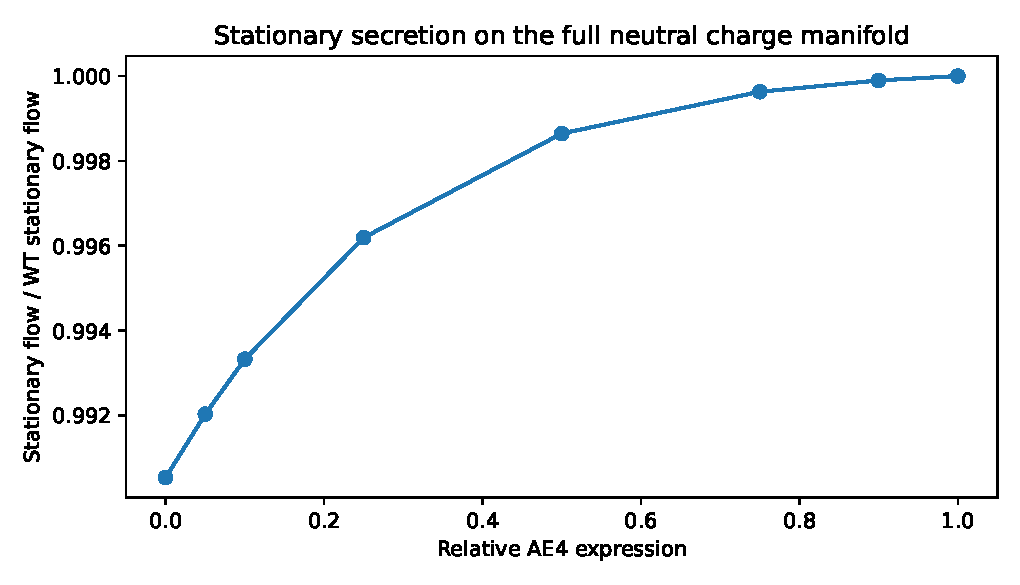
\includegraphics[width=.82\linewidth]{output/equilibrium_flow.pdf}
\caption{Constant stimulus C0 equilibrium secretion normalised by WT.
The vertical axis deliberately resolves the small change around one;
the complete null deficit is 0.94617\%, not the 600 s cumulative deficit.
Each point is a solved local root, not evidence of global uniqueness.}
\end{figure}
\begin{figure}[htbp]
\centering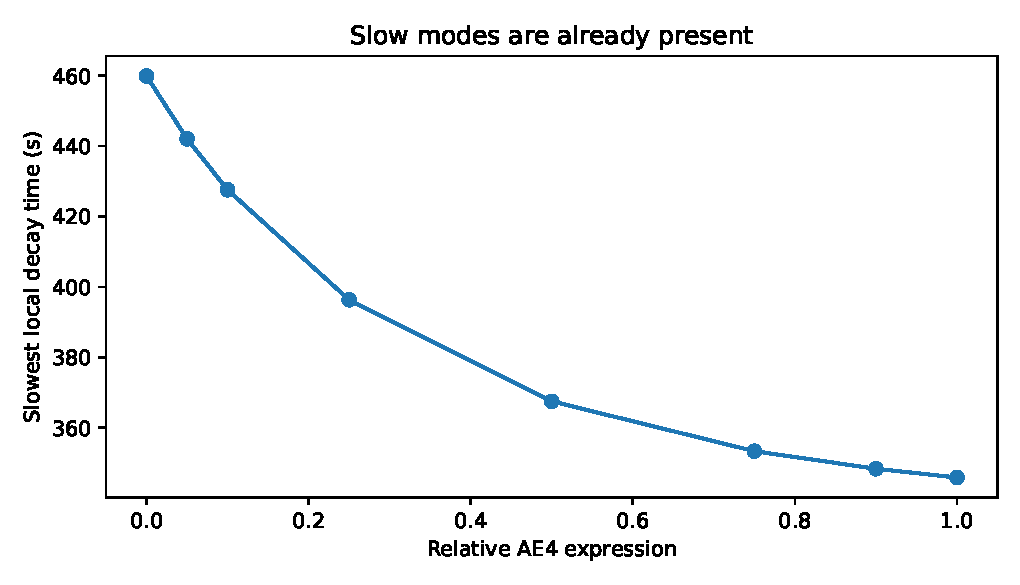
\includegraphics[width=.82\linewidth]{output/slow_modes.pdf}
\caption{Dominant local decay times on the eleven dimensional neutral
manifold during expression continuation. Carbon, alkalinity, both volumes,
finite lumen composition and regulation are retained. These local
timescales do not alone establish the shape of genotype divergence.}
\end{figure}
\begin{figure}[htbp]
\centering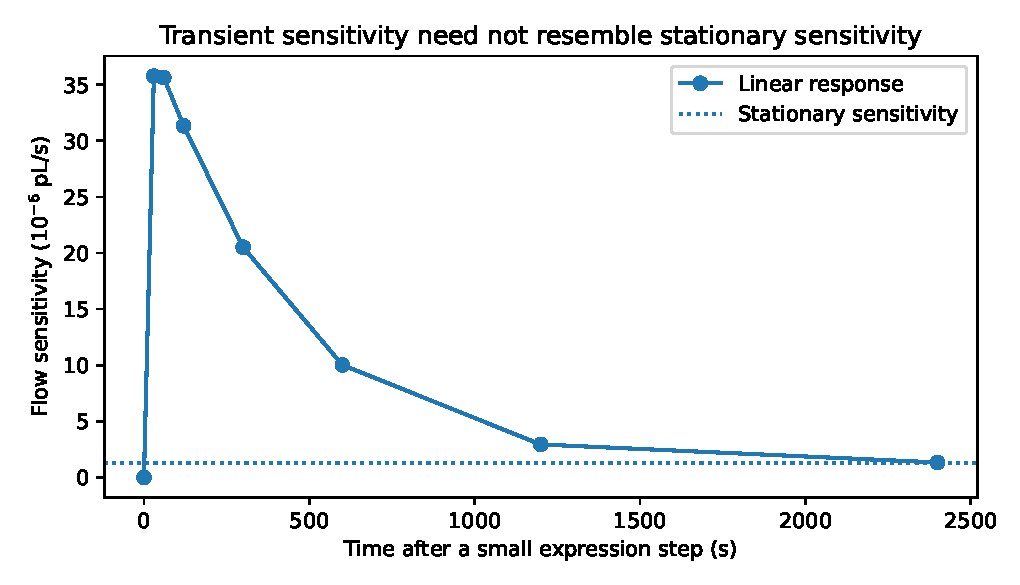
\includegraphics[width=.82\linewidth]{output/linear_response.pdf}
\caption{Local expression step response at the WT equilibrium.
This linear response retains input and secretion output projection.
It is a derivative experiment, not a replacement for a finite knockout
trajectory from the inherited resting state.}
\end{figure}
\FloatBarrier

\section{All frozen source classes}
The exact projections were derived above without class specific refitting.
For completeness, the full expression root of every class is tabulated here.
Sodium concentrations are in mM. Physiological acceptance and thermodynamic
compatibility are separate tests; passing this table's gates does not erase
the opposed fluxes reported in the spectral review.
\begin{center}\small
\begin{tabular}{lrrrl}
\toprule
Class & $\mathrm{pH}_i^*$ & $[\mathrm{Na}]_i^*$ & $t_{\mathrm{slow}}$ (s) & Failed criteria \\
\midrule
C0 & 7.0504 & 18.083 & 345.82 & None \\
C1 & 7.0139 & 45.694 & 564.38 & sodium \\
C2 & 6.5211 & 57.460 & 500.52 & sodium, pH \\
C3a & 7.0220 & 24.508 & 431.19 & None \\
C3b & 7.0734 & 14.206 & 314.61 & None \\
C4a & 6.5214 & 31.108 & 455.72 & pH \\
C4b & 6.5792 & 15.581 & 313.64 & pH \\
\bottomrule
\end{tabular}

\end{center}
In particular C0 is a physiological mathematical root with thermodynamic
opposition under the substituted ensemble source convention. Edge kinetics
inherited from the carrier are insufficient to guarantee consistency of
the whole substituted molecular cycle. The source vector analysis identifies
the conserved signatures that require measurement; it does not validate
the scalar kinetics for each molecular hypothesis.

\section{The prescribed Task 41 inverse family}
\label{sec:task41inverse}

The Task 41 construction is target selected. Its added hypothesis changes
stimulated CaCC conductance before the full electrical and NBC closure:
\begin{equation}
 g_{\mathrm{CaCC}}(e,a;\rho)
 =g_{\mathrm{parent}}\{1-a\rho(1-e)\},\qquad
 \rho=1-b,\quad 0\leq\rho<1.
 \label{eq:inversefamily}
\end{equation}
Here $e$ is AE4 expression and $a$ is the protocol normalised recruitment
fraction used by NBC:
\[
 a=\min\!\left\{1,\max\!\left\{0,
 \frac{[\mathrm{Ca}]_i-0.058\,\mu\mathrm M}{(0.25-0.058)\,\mu\mathrm M}
 \right\}\right\}.
\]
The parent CaCC Hill gate remains a distinct retained factor.
The full conserved system, carbonate closure, electrical closure, both
volumes and AE4 regulation remain active. WT nests the parent exactly for
every state and every $\rho$. At full activation, the null retains fraction
$b=1-\rho$ of its parent CaCC conductance.

Every 600 s trajectory uses the identical frozen WT initial conserved state
and original stimulus protocol. No genotype resting solve, new mechanism or
parameter fit is introduced. All inherited positivity, concentration, pH,
volume, source and conservation gates are checked at accepted solver endpoints
and at the original observation times. The original WT stimulation requirement
is also retained; it is not imposed retrospectively on mutants.

For $X\in\{\mathrm{A},\mathrm{S}\}$ define
\begin{equation}
 D_X(\rho,p)=1-\frac{I_{0,X}(\rho,p)}{I_{1,X}(p)}.
 \label{eq:inverseobservable}
\end{equation}
$I_{e,\mathrm A}$ is the adaptive time integral of outflow and
$I_{e,\mathrm S}$ is the original trapezoidal observable on integer seconds,
including $t=0$ and $10^{-6}$ s. These are distinct numerical observations.
The prescribed comparison threshold is $D_X=0.303$: it is one reported
standard error below the experimental mean of 35\%, whose reported standard
error is 4.7 percentage points. It is not a confidence limit, a measured
biological range or an admissibility gate.

\subsection{Reproduction and numerical crossing}
The selected Task 41 parameter is
$b=0.10511872843288446$, or $\rho=0.8948812715671155$.
The three selected trajectories reproduce the frozen sampled cumulative
outputs to within 6.7e-10 pL.
\begin{center}
\begin{tabular}{lrrr}
\hline
Case & Sampled output (pL) & Adaptive output (pL) & Sampled deficit (\%) \\
\hline
WT & 0.992524545 & 0.992544443 & 0 \\
5\% AE4 & 0.762622459 & 0.762624862 & 23.163365 \\
AE4 null & 0.692175197 & 0.692173709 & 30.261151 \\
\hline
\end{tabular}
\end{center}
In particular, the frozen selected null deficit is slightly below 30.3\%.
It must not be described as exactly attaining this new comparison threshold.

An ordered scan of 17 recruitment fractions, followed by bracketed numerical
root refinement in the prescribed family, gives:
\begin{center}
\begin{tabular}{lrrr}
\hline
Observable & Crossing $\rho$ & AE4 dependent recruitment (\%) & Residual $b$ \\
\hline
Adaptive & 0.8950726882 & 89.5072688 & 0.1049273118 \\
Original sampled & 0.8950806285 & 89.5080628 & 0.1049193715 \\
\hline
\end{tabular}
\end{center}
Both crossings pass every inherited 600 s gate. At the adaptive crossing,
the original sampled deficit is 30.2984507\%;
at the sampled crossing, the adaptive deficit is
30.3015492\%.
Refinement at relative solver tolerances $10^{-8}$ and $2\times10^{-9}$,
with respective maximum steps 2 s and 1 s, changes the two crossing fractions
by 1.4e-13 and
1.7e-11, respectively.
Independent integration of the 13 production states, followed by adaptive
quadrature of dense flow, also reproduces the selected cases and crossing.

The deficit increases at the sampled points, but monotonicity between them
and exclusion of all earlier unsampled crossings have not been proved.
These are the first numerical crossings found in this prescribed family,
not global lower bounds, universal recruitment requirements or independent
validation of the coupling hypothesis.

\subsection{The separate extension beyond 600 s}
Continuing constant full stimulation to 3600 s gives the following null
diagnostics. Each run passes all inherited gates through 600 s. Intracellular
pH is the only later gate failure; all other monitored gates continue to pass.
\begin{center}
\begin{tabular}{lrrr}
\hline
Case & First pH $=7.3$ time (s) & pH at 3600 s & Limiting local root pH \\
\hline
Selected Task 41 & 1486.30957 & 7.3117946 & 7.3120147 \\
Adaptive crossing & 1484.74517 & 7.3118437 & 7.3120644 \\
\hline
\end{tabular}
\end{center}
The limiting roots found from these late states are mathematical continuations
outside the inherited pH domain. They do not establish globally unique
equilibria or physiological long term validity. These separate diagnostics do
not change any frozen 600 s Task 41 result.

\subsection{Local uncertainty of the crossing}
For a locally regular numerical crossing with $\partial_\rho D_X\ne0$,
\begin{equation}
 \frac{\mathrm d\rho_X}{\mathrm d\log p}
 =-\frac{\partial_{\log p}D_X}{\partial_\rho D_X},\qquad
 \frac{\mathrm d\log b_X}{\mathrm d\log p}
 =-\frac{1}{1-\rho_X}\frac{\mathrm d\rho_X}{\mathrm d\log p}.
 \label{eq:thresholdsensitivity}
\end{equation}
Eight effective or architecture derived quantities were selected using the
Task 43 provenance classification. A perturbed WT denominator is used with
the same perturbed parameter in the null. The conserved initial state is
always held at the inherited WT value. Thus changing the buffer amount also
changes the algebraic initial pH; it does not trigger a new resting solve.

The following elasticities refer to the adaptive crossing. The companion
sampled results are retained in the machine readable crosswalk.
\begin{center}
\begin{tabular}{lrr}
\hline
Parameter & $\mathrm d\log\rho/\mathrm d\log p$ & $\mathrm d\log b/\mathrm d\log p$ \\
\hline
NBC capacity & -0.0059550 & +0.0507982 \\
AE4 carrier amount & -0.0050569 & +0.0431371 \\
NKCC effective scale & -0.0021926 & +0.0187041 \\
NHE1 carrier amount & +0.0008018 & -0.0068396 \\
Pump capacity & -0.0355825 & +0.3035333 \\
CaCC conductance & +0.0983320 & -0.8388120 \\
Cell buffer amount & +0.0071557 & -0.0610411 \\
Apical water permeability & -0.0002975 & +0.0025380 \\
\hline
\end{tabular}
\end{center}
The derivative calculation is checked against independently solved nearby
crossings at logarithmic perturbation sizes $10^{-3}$ and $5\times10^{-4}$.
Every perturbed WT and null trajectory passes its inherited gates. The maximum
relative discrepancy between implicit crossing derivatives and nearby root
differences is 1.7e-06.
The larger relative sensitivity of residual recruitment $b$ is relevant when
interpreting a conductance assay. None of these eight quantities has an
established experimental uncertainty interval in the audited configuration.
Accordingly, these calculations establish local sensitivity only; they do
not prove robustness over a finite range or identify a finite parameter
change that overturns the conclusion.

\subsection{A discriminating experiment and scope}
At the numerical comparison crossing the null must retain approximately
10.49\% of stimulated CaCC conductance in this family. A direct test would
compare stimulated CaCC conductance and channel recruitment in WT and AE4
loss cells while matching calcium activation, voltage, intracellular chloride
and pH, so that a changed driving force is distinguished from a changed
conductance. Surface channel abundance and channel open probability would
help distinguish recruitment from gating. Concurrent measurements of pH,
chloride, cell volume and secretion over the first ten minutes and after
approximately 25 minutes would test the predicted coupled response and its
later pH failure. A secretion measurement alone does not identify this
specific dependency.

\begin{figure}[htbp]
\centering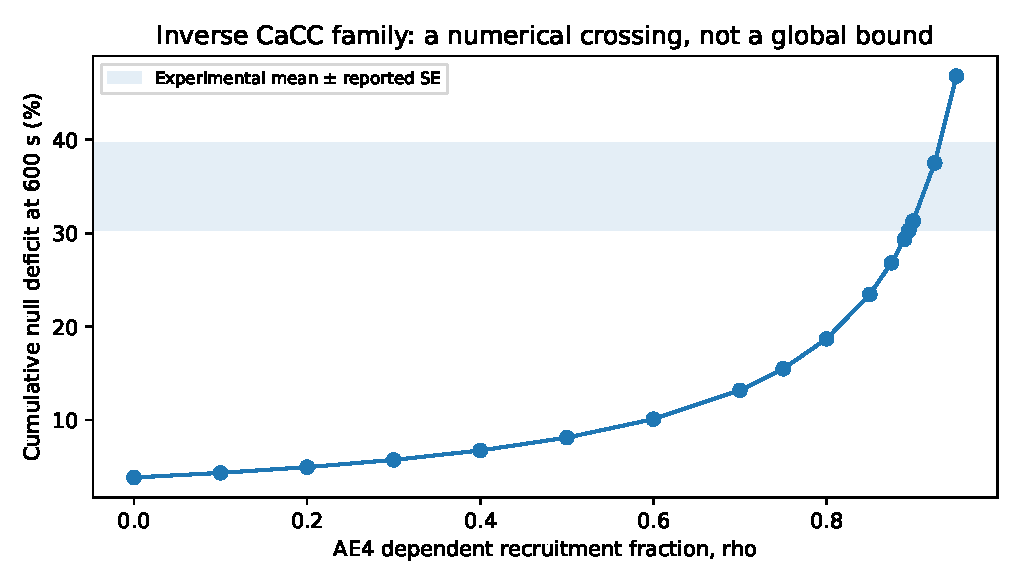
\includegraphics[width=.82\linewidth]{output/inverse_threshold.pdf}
\caption{Ordered numerical scan within the one prescribed Task 41 family.
The experimental band represents the reported mean plus or minus one
standard error, not a confidence interval. The refined adaptive and sampled
crossings are recorded separately. Neither a global lower bound nor global
monotonicity follows from the plotted points.}
\end{figure}
\begin{figure}[htbp]
\centering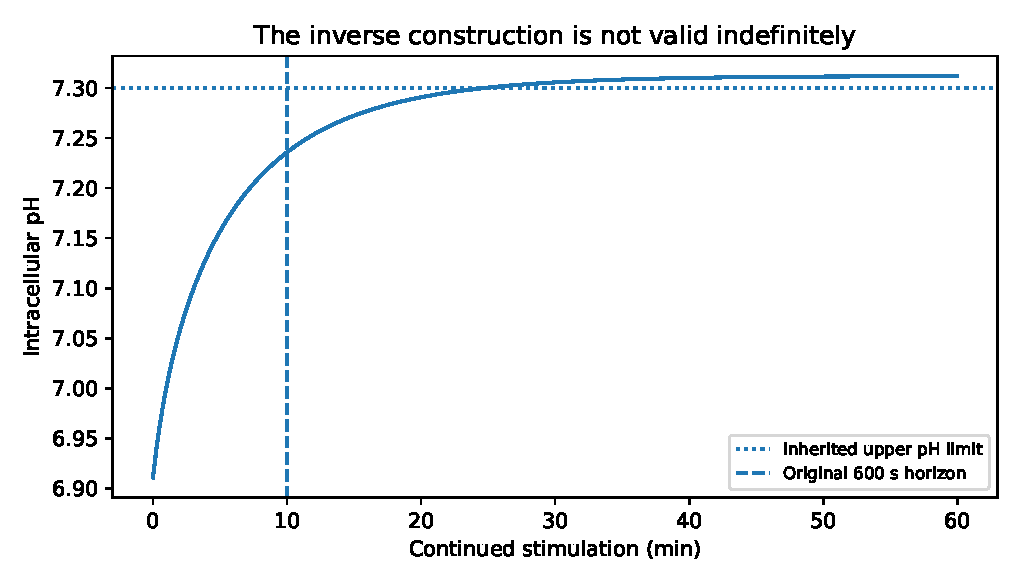
\includegraphics[width=.82\linewidth]{output/inverse_ph.pdf}
\caption{Separate extension of the adaptive crossing null beyond the
declared 600 s Task 41 window. It first crosses the inherited upper pH
gate near 1485 s; the selected case has a nearly identical late crossing.
The later diagnostic does not revise the frozen 600 s
observable; it limits claims of sustained physiological validity.}
\end{figure}
\FloatBarrier

\section{Dependence on uncertain parameters}
\subsection{Sensitivity crosswalk with Task 43}
The sixteen selected parameters are uncertain effective settings or inherited calibrated capacities. Each is perturbed independently by $p\exp(\pm h)$, with $h=10^{-3}$ and $5\times10^{-4}$; both genotypes are solved afresh at each perturbed point. These steps are numerical checks and do not define uncertainty intervals. No defensible physiological interval is available from the provenance audit, so no global robustness claim is made.
\begin{center}\small
\begin{tabular}{lrrrrr}\hline
Parameter & $E_Q$ & $\partial\mathrm{pH}/\partial\log p$ & $E_D$ & $E_{C_N}$ & $E_{\tau_{\rm WT}}$\\\hline
NBC capacity & 0.01992 & 0.06483 & 2.085 & -0.06438 & 0.107\\
AE4 amount & 0.0008114 & -0.07246 & 0.08494 & 0.02339 & -0.06397\\
NKCC scale & 0.05536 & -0.001558 & -1.494 & 0.06404 & 0.1901\\
NHE amount & -0.003261 & 0.07084 & -0.2293 & 0.007679 & -0.01473\\
Pump capacity & 0.5259 & 0.1206 & 4.634 & -0.2734 & -1.522\\
CaCC conductance & 0.03247 & -0.005524 & -0.2212 & 0.01105 & 0.008274\\
Cell buffer amount & -0.001575 & 0.001396 & -0.2063 & 0.009504 & 0.3086\\
Apical water permeability & 0.002129 & -8.317e-05 & -0.003558 & 0.0002239 & -3.74e-05\\
AE4 activation time & 0 & 0 & 0 & 0 & 0\\
AE4 activation gain & 0.0001623 & -0.01449 & 0.01699 & 0.004678 & -0.01279\\
Apical pump fraction & 0.04956 & -0.003571 & -0.05983 & 0.003151 & 0.04517\\
NHE stimulation gain & -0.003261 & 0.07084 & -0.2293 & 0.007678 & -0.01473\\
Basolateral CO$_2$ permeability & -0.004448 & -0.08319 & -0.4338 & 0.05062 & -0.06818\\
AE2 capacity & -7.335e-05 & 0.000363 & -0.03056 & -0.03383 & 7.508e-05\\
NBC saturation width & -0.01435 & -0.0467 & -1.502 & 0.01777 & -0.07263\\
NKCC stimulation gain & 0.05536 & -0.001558 & -1.494 & 0.06404 & 0.1901\\
\hline\end{tabular}\end{center}
Here $E_Y=\partial\log Y/\partial\log p$ and $D=1-Q_{\rm null}/Q_{\rm WT}$ is the stationary deficit. Its small baseline value makes $E_D$ potentially large; the machine readable table also supplies percentage point derivatives. pH is already logarithmic, so its unnormalised derivative is shown; the hydrogen concentration elasticity is $-\log(10)\partial\mathrm{pH}/\partial\log p$. All derivatives are partial sensitivities at the inherited parameter point, without recalibration.
Pump capacity has the largest local effect on WT secretion and on the stationary null deficit. The latter is also sensitive to NBC capacity and its assumed saturation width, and to effective NKCC capacity. These are priorities for experimental constraint. The calculations do not show that a finite parameter change overturns a conclusion, and cannot establish that the small null phenotype persists throughout an unknown uncertainty range. The exact balance identities survive these capacity changes within the specified architecture; their numerical consequences need not.
The equilibrium total alkalinity support ratio is identically one and cannot demonstrate robustness. The saved results instead give the NBC share $J_B/J_4$, the observed non NBC share $(J_H-J_2)/(2J_4)$, and a conditional capacity ratio $(H_{\max}+J_{2,\max})/(2J_4)$. The bound assumes the fixed bath, positive sodium and $\mathrm{pH}_i\geq6.6$. It permits AE2 to supply alkalinity at its maximal reverse capacity. Its local sensitivity is useful, but it does not prove the available capacity over an unknown parameter interval.
The AE4 activation time has no local effect on constant stimulus equilibria. Its eigenvalue is $-1/\tau_4$ and is separated from the slower chemical mode at this point; a zero local slow mode sensitivity does not establish that activation timing is irrelevant to finite time secretion. The buffer calculation holds the fixed charge and impermeant osmole pools fixed while changing only buffer amount. NKCC capacity and its stimulated multiplier produce the same stationary perturbation because only their product enters at constant full stimulation.
Independent root perturbations validate the IFT derivatives at both steps, and expression perturbations validate the chloride compensation gain at both steps for every nearby parameter point. Fixed state parameter derivatives use the smaller steps $10^{-5}$ and $5\times10^{-6}$ to resolve cancellation in the buffer response. Decay sensitivities additionally use fourth order differentiation of the chemical block at two steps, together with the exact regulatory eigenvalue; the block triangular structure retains all eleven dynamical eigenvalues. The supplied files retain root residuals, physiological gate results, Jacobian step checks and all derivative comparisons. The separate inverse family calculation supplies the Task 41 crossing sensitivity.

The independent complete gate supplement resolves all 128 perturbed WT
and null parameter roots and 256 additional expression roots used to
check compensation. Every numerical solve succeeds and every inherited
gate passes. Its largest conservation residual divided by its own tolerance
is $4.086\times10^{-5}$; the largest independent RHS residual is
$6.880\times10^{-12}$. This supplements the original derivative checks
without weakening a gate. Exact reproduction of this supplementary
calculation from the clean numerical checkout is recorded separately.

% Primary source audit, completed 15 September 2026.
% 2015: PMC4409235 full primary HTML, Experimental Procedures (Statistical
% Analyses), Results, Table 1 and Figures 1--2; retrieved with urllib after
% the web reader returned a CAPTCHA. SHA256 of retrieved HTML:
% 72dd59caaede1c477c643f818926390bf48e2966692b4dbd47b752b4f6fbe98d.
% 2018: literature/core/2018_AE4_model.pdf, pp. 258--263, 269--271;
% SHA256 e2782a89b13a6dd27ea1c510d11515bacc33931697baccb678802de47bb13a23.
% 2021: primary PubMed record 34585968, abstract and Figures 1--2 captions;
% the complete article was not required or claimed to be reread.
% 2025: PMC12463136 primary author manuscript, Methods, Results and Discussion;
% retrieved HTML SHA256:
% 890c6f4b9834e8f0c8683e181aac5c8e3d49e045d7ada3d728b1b0cc591c2583.
% No source text or protected manuscript text is copied into this section.
\section{Comparison with experimental evidence}
\label{sec:literature-comparison}

\paragraph{The gland phenotype and the comparison threshold.}
In the 2015 mouse submandibular gland study, stimulation used
$0.3\,\mu\mathrm{M}$ carbachol and $5\,\mu\mathrm{M}$ isoproterenol.
AE4 deletion reduced total secretion over ten minutes by
$35\pm4.7\%$ (mean $\pm$ standard error; six glands per genotype).
Initial flow over two to three minutes was comparable, with the deficit
developing later. AE2 deletion had no detectable flow effect against its
own control strain. AE4 deficient acinar cells had lower resting chloride
and slower chloride reuptake; initial chloride exit and resting pH were
not detectably changed. These are distinct measurements, rather than
interchangeable manifestations of a single steady flux~\cite{Pena2015}.
The prescribed $30.3\%=35\%-4.7\%$ inverse target is therefore a
comparison value one reported standard error below the mean. It is not
a confidence bound, an uncertainty interval for a model parameter, or
a universal biological minimum.

The Task 40 cumulative null deficit of $3.8575\%$ establishes a small
effect for the frozen model and protocol. The equal routing identity
does not establish that small magnitude for every admissible parameter
choice. Nor does agreement at $600\,\mathrm{s}$ establish the observed
time course. The present simulations initialise every genotype at the
inherited WT resting state, whereas the experiment used established
knockout animals. That difference should remain explicit when comparing
the initial response or stored intracellular chloride.

\paragraph{Compensation and pH.}
The 2015 isolated NKCC1 assay used bicarbonate free solution,
$30\,\mu\mathrm{M}$ ethoxyzolamide and
$50\,\mu\mathrm{M}$ T16Ainh-A01; bumetanide identified the
NKCC1 dependent component. Initial chloride uptake showed no detectable
genotype difference. Stimulation induced NHE dependent alkalinisation
also showed no genotype difference~\cite{Pena2015}.
Neither finding measures the complete stimulated network integral.
Consequently, the approximately $23.16\%$ rise in integrated NKCC1
loading in the frozen Task 40 null is an unresolved experimental
tension. It must not be described as observed compensation. The local
equilibrium compensation derivative, the relative integrated NKCC1
increase and the fraction of missing AE4 chloride replaced by NKCC1
are three separate quantities throughout this report. Unchanged assay
alkalinisation does not establish equal NHE1 net flux at different ionic
states, and unchanged resting pH does not identify individual alkalinity
sources. A discriminating experiment would measure chloride loading,
pH, sodium and volume through the same combined stimulus, with
pathway specific perturbations and parallel controls.

\paragraph{What the 2018 model actually established.}
The published model predicted an approximately $24\%$ flow reduction
after AE4 deletion. Its reduced flow settled within about two minutes;
the authors explicitly contrasted this with experimental development
over roughly ten minutes. It predicted little NKCC1 activation following
either exchanger deletion. It included carbon dioxide hydration, NHE1,
AE2 and AE4, without another proton or bicarbonate transporter, and
held lumen volume constant~\cite{VeraSiguenza2018}.
Those are historical model properties, not experimental determinations
of the full network. The present retained carbon, alkalinity and volume
coordinates make the storage terms explicit. Numerical slow modes and
their projection onto secretion must be examined before attributing a
temporal discrepancy to absent slow regulation. A slow eigenvalue alone
does not reproduce delayed genotype divergence.

\paragraph{Regulation and the inverse CaCC family.}
The 2021 study found that beta adrenergic stimulation increased native
AE4 activity, that H89 prevented the response, and that constitutively
active PKA increased AE4 activity in CHO cells. The S173A mutant lost
PKA activation, whereas S273A retained it. The authors described
phosphorylation of S173 as a probable mechanism; H89 is a nonselective
inhibitor~\cite{Pena2021}.
This supports regulated AE4 activity, but does not measure the model's
AE4 regulatory gain, relaxation time or an AE4 to CaCC recruitment law.
The Task 41 inverse crossing quantifies a requirement within one family
selected using the phenotype. It supplies no independent validation of
that family. Its direct experimental test is the fraction of stimulated
apical chloride conductance lost upon AE4 perturbation at matched
calcium, membrane potential, chloride, pH and volume, resolved from the
initial response into sustained secretion. This distinguishes altered
channel recruitment from changed driving force and from intracellular
chloride storage.

\paragraph{Molecular source classes.}
Catal\'an and colleagues studied human AE4 expressed in HEK293 cells,
combining mutagenesis, transport assays and molecular dynamics. The
T756A--T448I mutant lost transport with extracellular sodium while
retaining activity with potassium. Their discussion proposes both
bicarbonate and carbonate cycles, including exchanged sodium and
potassium, and explicitly calls for further experiments to resolve
the alternatives~\cite{Catalan2025}.
Thus the seven frozen classes are specified source hypotheses, not seven
experimentally established full cycles. Their conserved projections
and equilibrium tests separate chloride, carbon, alkalinity and charge
consequences under inherited scalar kinetics. Matching one projected
signature cannot establish identical molecular mechanisms or identical
whole cell responses. An unsuccessful root search cannot establish
nonexistence. A thermodynamically opposed or nonphysiological case must
retain that qualification. Joint measurements of cation and anion
flux ratios, reversal conditions and current would constrain the source
vector; rates measured across those gradients would constrain the
separate kinetic law.

\paragraph{The most urgent missing measurements.}
The evidence checked here does not establish the identity, abundance
or capacity of the assumed inward $1\mathrm{Na}:2\mathrm{HCO}_3$
pathway. The alkalinity proposition gives a conditional requirement for
additional support when the admissible NHE1 and AE2 contribution is
insufficient. It does not prove that a particular NBC isoform is
universally necessary. The assumed loading allocation used to construct
NBC capacity is not a measured transporter partition.
Measurements of sodium and bicarbonate influx with current and pH
during combined stimulation are therefore a priority, alongside native
NHE1 and NKCC1 capacity and state dependence. The sensitivity crosswalk
identifies which effective capacities, conductances and buffer settings
matter most at the analysed point. Until independent ranges constrain
them, local elasticities do not establish robustness over biological
uncertainty.

\paragraph{Scope of source verification.}
The comparison uses the 2015 primary full text and Figures 1 and 2,
the repository copy of the 2018 published paper, the 2021 primary
abstract and figure captions, and the 2025 primary author manuscript
including its discussion. These four references were checked to that
extent. No systematic literature survey, new experimental measurement
or complete source audit of every inherited kinetic coefficient is
claimed here; parameter provenance is recorded separately in Task 43.


\clearpage
\section{What is established and what remains unresolved}
\begin{longtable}{p{.17\linewidth}p{.76\linewidth}}
\toprule
Status & Conclusion and scope\\\midrule
\endhead
Proved or exact & Unique mathematical carbonate and electrical roots under
the stated positivity and slope assumptions, smooth dependence inside strict
executable brackets, local well posedness, exact retained nondimensionalisation,
alkalinity storage budget, conditional capacity obstruction and equal routing
chloride identity. Joint source projections have rank five.\\
Local numerical & Twenty six class/expression cases yield nonsingular stable
local roots; twenty two pass the physiological gates. WT/null slow times are
345.82/459.92 s. The stationary null deficit is 0.94617\%; the WT local
chloride compensation is 92.901\%. Local IFT and parameter derivatives
are independently verified. A physiological NBC absent equilibrium exists.\\
Finite time numerical & Frozen Task 40 observables reproduce. The 60--600 s
integrated NKCC increase is 23.163\% and missing AE4 chloride compensation
88.507\%. First numerical Task 41 crossings need about 89.51\% AE4 dependent
stimulated CaCC recruitment. The 600 s gates pass; selected continued null
cases later violate the pH gate.\\
Unresolved & Global uniqueness, stability and positivity; a justified reduced
model; global exclusion of earlier inverse crossings; robustness over unknown
parameter ranges; native carrier abundance and pathway identity; molecular
source stoichiometry and compatible kinetics; the isolated NKCC assay tension;
independent validation of the Task 41 CaCC coupling.\\\bottomrule
\end{longtable}

Several earlier interpretations require explicit correction. Stationary
cancellation does not imply zero total sensitivity or a uniformly small
phenotype. The system already contains slow chemical modes; the corrected
regulatory derivative gives 30 s, not the spurious 60 s obtained by crossing
the production clamp. The initial unsuccessful continuation record is not
evidence of nonexistence. NBC is not universally necessary for secretion
in this frozen system, though it supplies most of the larger AE4 alkalinity
demand. The old selected Task 41 point gives a sampled deficit of
30.26115\%, slightly below 30.3\%, and the refined crossing depends on
the declared integral. The comparison value is mean minus one standard
error. The construction remains target selected and its late pH failure
must accompany any claim about sustained stimulation.

The immediate experimental priorities are functional pump capacity and
apical distribution; NBC equivalent sodium/bicarbonate flux, current and
its saturation curve; ion conditioned NKCC and NHE capacity; simultaneous
TIC, buffering, pH and volume measurements; and stimulated CaCC conductance
and recruitment under acute AE4 perturbation at matched calcium and driving
forces. Source stoichiometry requires combined cation, chloride, carbon and
current measurements. These measurements would constrain the effective
parameters that dominate local sensitivities and separate a transport
pathway from a fitted phenomenological coupling. An accepted physiological
point and small numerical perturbations do not supply those missing ranges.

\section{Reproduction, verification and deliverables}
All new material is under \texttt{analysis/44\_full\_system\_mathematics/}.
The frozen scientific base is
\nolinkurl{c4d4f207f702d8eee09ab94d2d90ae90552dd641}.
The original source manifest, active parameter objects, source hashes and
recovery record distinguish scientific files from historical metadata changes.
The complete numerical checkpoint was cloned independently, checked out
detached, and regenerated with empty inverse trial caches before this
standalone report was written. All eighteen commands passed. Forty six
regenerated authoritative JSON/CSV files plus one unchanged historical
record were compared: all 331157 numeric values matched bit for bit.
Only elapsed runtime and an ancestor validated verification commit field
were excluded. All 532 inverse trial files were regenerated; the optional
cache is not part of the published scientific deliverables. All 1751 tracked
files outside Task 44 were unchanged in that clean replay.

\begin{longtable}{>{\raggedright\arraybackslash}p{.42\linewidth}>{\raggedright\arraybackslash}p{.51\linewidth}}
\toprule
File or group & Content\\\midrule\endhead
\texttt{README.md}, \texttt{RECOVERY.md} & Reproduction commands, recovered
history and derivative correction.\\
\texttt{core.py}, \texttt{run\_analysis.py} & Exact coordinates, production
adapter, scaling, continuation, local derivatives and baseline reproduction.\\
\texttt{verify\_exact.py} & Independent full RHS reconstruction, pH and
electrical closure checks, exact source and balance identities at valid states.\\
\texttt{equilibrium\_review.py} & Full physiological gates, matched
eigenvalues, modal projection and independent nearby roots.\\
\texttt{sensitivity\_analysis.py} & Sixteen uncertain parameter sensitivities
and derivative verification; Task 43 crosswalk source.\\
\texttt{verify\_sensitivity\_gates.py} & All 384 nearby roots tested against
the complete inherited gates, with solver failures retained separately.\\
\texttt{inverse\_analysis.py}, \texttt{inverse\_verify.py} & Original family,
both crossing observables, long diagnostics, eight parameter sensitivities
and independent thirteen state integration/quadrature.\\
\texttt{output/}, \texttt{inverse\_detail/} & Machine readable source audit,
scales, trajectories, roots, spectra, derivatives, projections, crossing scan,
refinement, gates and verification.\\
\nolinkurl{output/clean_recomputation_verification.json} & Exact numerical
checkpoint, commands, file comparisons, exclusions and protected file audit.\\
\texttt{report.tex}, \texttt{build.sh}, \texttt{sources.bib} & Standalone
report source, bibliography and clean build command.\\
\texttt{FINAL\_STATUS.md} & Final verified checkpoint, findings, failures,
caveats, artifact paths and checksums.\\\bottomrule
\end{longtable}

The PDF build resolves every citation and reference. Figures are generated
from saved verified results; axis ranges and the distinct observables are
stated in captions. The report, TeX fragments, vector figures and complete
machine readable outputs are retained for scientific review. No model
source, frozen output, Task 1--42 analysis or manuscript text was changed.
The two analysis branches remain separate and unmerged.

\bibliographystyle{plain}
\bibliography{sources}
\end{document}
